\clearpage
\newpage
\noindent\\
\thispagestyle{empty}
\begin{center}
\Large
\begin{flushright}
\vspace{17cm} {\Huge \em{ \textbf{\textcolor{ultramarine}{CURSOS}}}} \\ [0.5cm]
\addcontentsline{toc}{section}{Cursos}
\end{flushright}
\normalsize
\end{center}

\small
\clearpage
\pagestyle{fancy}
\SetHeader{Cursos}{\textit{Congreso Interamericano de Estadística}}

%\newcommand{\titulo}{algo}
%\newcommand{\presentador}{algo}
%\newcommand{\lugar}{algo}

 %--------------------------------------------------------------------------
\renewcommand{\titulo}{DEFINITIVE SCREENING AS A SYSTEM FOR EXPERIMENTAL DESIGN AND OPTIMIZATION}
\renewcommand{\presentador}{DR. CHRISTOPHER J. NACHTSHEIM}
\renewcommand{\lugar}{UNIVERSITY OF MINNESOTA, USA}
\addcontentsline{toc}{subsubsection}{\titulo. \presentador}
\vspace*{1cm}

\begin{center}
\textbf{\textcolor{ultramarine}{\titulo \\}}
\bigskip
\textit{\presentador \\}
\bigskip
\scriptsize{\lugar}
\bigskip
\end{center}

\noindent Since their introduction by Jones and Nachtsheim in 2011, Definitive Screening Designs (DSDs) have seen application in fields as diverse as bio-manufacturing, green energy production, medical technology, laser etching, and touch screen optimization. DSDs are small, three-level screening designs that frequently allow the experimenter to perform factor screening and subsequent response-surface optimization in a single step. Moreover, the capabilities of this new family of designs has expanded considerably in the interim. We now understand that definitive screening designs can be easily constructed from conference matrices; we know how to add two-level categorical factors; we know how to block these designs orthogonally; and an effective model selection method, that leverages the unique structure of DSDs, has been developed. In this short course, we will review these developments and illustrate the use of the designs with several real-world applications.

\begin{table}[H]
\centering
\begin{tabular}{m{0.25\textwidth}  m{0.7\textwidth}}
\begin{center} 
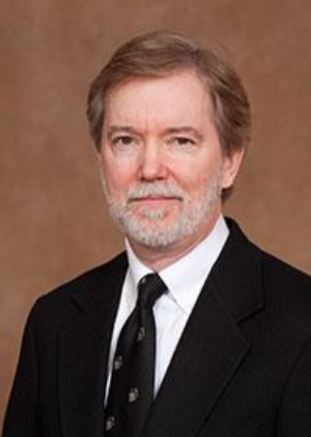
\includegraphics[width=0.2\textwidth]{./fotos/chris} \end{center} & 
\noindent \small{Christopher J. Nachtsheim. Licenciado en Matemática y Métodos Cuantitativos, Master en Investigación Operativa y Estadística y PhD en
Investigación Operativa. Es profesor y director de Operations Management (Gerenciamiento Operativo) en el departamento Supply Chain and Operations Management,
en Carlson School of Management de la University of Minnesota. Fue director de dicho departamento entre los años 2000 y 2015. Las áreas de expertise del Dr.
Nachtsheim son Diseño de Experimentos, Análisis de Regresión de la Variancia y Métodos de Mejora de la Calidad. Entre sus publicaciones se encuentran los libros
“Applied Linear Statistical Models”, 5ta ed., 2005, y “Applied Linear Regression Models”, 4ta ed., 2004, escritos con coautoría de John Neter, Michael Kutner, y William Li. El Dr. Nachtsheim ha publicado más de 70 artículos en la literatura estadística; ha colaborado como editor asociado con muchas revistas científicas en
esta área incluyendo Journal of the American Statistical Association, Technometrics, Journal of Quality Technology, Statistics and Computing, y Journal of Statistical Computation \& Simulation; ha sido galardonado con varios premios: Brumbaugh de la American Society of Quality (ASQ) al mejor artículo publicado en el área de control de calidad industrial (1991, 2009, 2012 y 2015), Lloyd S. Nelson de ASQ al artículo con mayor impacto en los profesionales (2010 y 2012) y Jack Youden a la mejor comunicación expositiva publicada en Technometrics (2011), entre otros. Ademas, él es miembro de la American Statistical Association.} \\
\end{tabular}
\end{table}

 %--------------------------------------------------------------------------
\newpage
\clearpage
\renewcommand{\titulo}{INTERLOCUTORES DE LOS SISTEMAS ESTADÍSTICOS NACIONALES EN EL MARCO DE LA CALIDAD EN LAS ESTADÍSTICAS OFICIALES}
\renewcommand{\presentador}{DRA. MARCIA QUINTSLR}
\renewcommand{\lugar}{INSTITUTO BRASILEIRO DE GEOGRAFIA E ESTADÍSTICA, BRASIL}
\addcontentsline{toc}{subsubsection}{\titulo. \presentador}
\vspace*{1cm}

\begin{center}
\textbf{\textcolor{ultramarine}{\titulo \\}}
\bigskip
\textit{\presentador \\}
\bigskip
\scriptsize{\lugar}
\bigskip
\end{center}

\noindent El análisis del concepto de "gobernanza", como propulsor de la transparencia y de la rendición de cuentas, en todas las etapas del proceso de producción y en la utilización de las estadísticas oficiales es la motivación central para el curso propuesto. La gobernanza implica una interacción intensiva con las diversas partes interesadas en los SEN. Se comenta el escenario global de la dimensión informacional y la presencia correspondiente de la gobernanza. Un elemento que conecta este panorama general con el escenario mundial de las estadísticas oficiales es el contexto de la "revolución de los datos". En este escenario estadístico global, se destacan las repercusiones de la Agenda 2030 para el Desarrollo Sostenible y el nuevo preámbulo de los Principios Fundamentales de las Estadísticas Oficiales, a partir de la mención explícita a las acciones de la rendición de cuentas. Los interlocutores y las acciones de gobernanza propuestas en el marco de la calidad estadística se presentan bajo el punto de vista empírico. En el campo teórico se explora, bajo el enfoque de la ética informativa, los valores de la transparencia y de las buenas práticas de gobernanza.

\begin{table}[H]
\centering
\begin{tabular}{m{0.25\textwidth}  m{0.7\textwidth}}
\begin{center} 
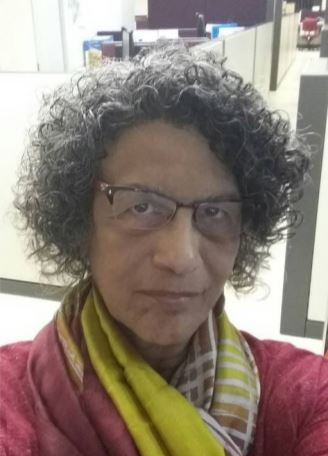
\includegraphics[width=0.2\textwidth]{./fotos/marcia} \end{center} & 
\noindent \small{Marcia Quintslr es brasileña, tiene experiencia en el diseño, planeamiento, producción, análisis y gestión en Estadísticas Oficiales. En el Instituto Brasileño de Geografía y Estadística (IBGE) actuó, desde octubre de 2011 hasta abril de 2014, coordinando la Dirección de Encuestas del Instituto, área responsable por el plan estadístico brasileño y por la Coordinación de las Encuestas de Hogares (2006-2011). Su formación académica es en matemática – ciencia de la computación, con posgrado en estadística. Actualmente está cursando una Maestría en Ciencia de la Información en el Instituto Brasileiro de Ciência e Tecnologia y Universidade Federal do Rio de Janeiro, donde realiza investigación sobre estadísticas, política de información, poder y representación del
conocimiento sobre la sociedad.} \\
\end{tabular}
\end{table}

 %--------------------------------------------------------------------------

\newpage
\clearpage
\renewcommand{\titulo}{INTRODUCCIÓN A R-INLA. AJUSTE DE MODELOS ESPACIALES Y ESPACIOTEMPORALES A DATOS DE ÁREA CON APLICACIONES EN \mbox{EPIDEMIOLOGÍA}}
\renewcommand{\presentador}{DRA. MARÍA DOLORES UGARTE}
\renewcommand{\lugar}{UNIVERSIDAD NACIONAL DEL LITORAL, ARGENTINA}
\addcontentsline{toc}{subsubsection}{\titulo. \presentador}
\vspace*{1cm}

\begin{center}
\textbf{\textcolor{ultramarine}{\titulo \\}}
\bigskip
\textit{\presentador \\}
\bigskip
\scriptsize{\lugar}
\bigskip
\end{center}

\noindent El enfoque Bayesiano resulta particularmente útil para modelizar conjuntos de datos espaciales y espacio-temporales debido a su gran flexibilidad para construir modelos complejos. Sin embargo, los procedimientos de inferencia MCMC (métodos de Monte Carlo basados en cadenas de Markov) pueden ser computacionalmente prohibitivos. En este curso se presentará un método alternativo para realizar inferencia Bayesiana basado en aproximaciones de Laplace e integración numérica. Para implementar el método utilizaremos el paquete R-INLA y ajustaremos algunos modelos espaciales y espacio-temporales en el ámbito de la representación cartográfica de enfermedades (disease mapping).

\begin{table}[H]
\centering
\begin{tabular}{m{0.25\textwidth}  m{0.7\textwidth}}
\begin{center} 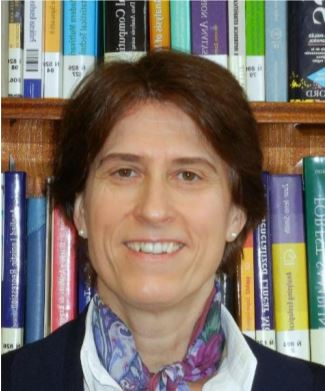
\includegraphics[width=0.2\textwidth]{./fotos/ugarte} \end{center} & 
\noindent \small{María Dolores Ugarte es licenciada en Matemáticas por la Universidad de Zaragoza y Doctora en Ciencias Matemáticas por la Universidad Pública de
Navarra (UPNA). Realizó su formación posdoctoral en el Departamento de Matemáticas y Estadística de la Universidad Simon Fraser (Canadá). Actualmente es catedrática de universidad del área de Estadística e Investigación Operativa de la Universidad Pública de Navarra (Pamplona, España). Sus líneas principales de investigación se enmarcan en el contexto de la estadística espacial y espacio-temporal y en el campo general de la estimación en áreas pequeñas. Actualmente es
(co)-editora jefe de la revista TEST, miembro del Consejo Ejecutivo de la Federación Europea de Sociedades de Estadística (FenStat) y colaboradora de la División de Coordinación, Evaluación y Seguimiento Científico Técnico de la Agencia Estatal de Investigación del Ministerio de Economía, Industria y Competitividad de España.} \\
\end{tabular}
\end{table}

 %--------------------------------------------------------------------------

\newpage
\clearpage
\renewcommand{\titulo}{MODELOS DE MAPEO ASOCIATIVO EN INFO-GEN}
\renewcommand{\presentador}{DRA. CECILIA BRUNO y DRA. ANDREA PEÑA MALAVERA}
\renewcommand{\lugar}{UNIVERSIDAD NACIONAL DE CÓRDOBA, ARGENTINA.}
\addcontentsline{toc}{subsubsection}{\titulo. \presentador}
\vspace*{1cm}

\begin{center}
\textbf{\textcolor{ultramarine}{\titulo \\}}
\bigskip
\textit{\presentador \\}
\bigskip
\scriptsize{\lugar}
\bigskip
\end{center}

\noindent Info-Gen es un Software estadístico para análisis de datos genéticos (Balzarini y Di Rienzo, 2004), en su interface con el software R permite estimar diferentes modelos propuestos en estudios de mapeo asociativo (MA), una técnica introducida en los estudios de mejoramiento genético para identificar genes responsables de la variación de caracteres cuantitativos. El MA se usa en el mejoramiento de especies vegetales para identificar regiones genómicas asociadas a caracteres fenotípicos de herencia compleja como rendimientos y componentes de rendimiento. Los loci que se asocian con cambios, estadísticamente significativos, de estos caracteres cuantitativos son denominados Quantitative Trait Loci (QTL). En el análisis clásico de QTL las poblaciones de mapeo son experimentalmente creadas mientras que el MA puede implementarse a partir de colecciones de germoplasma no diseñadas ad-hoc, este hecho ha promovido la adopción de la técnica en estudios de asociación. En este cursillo se introducirá el uso de modelos de mapeo de asociaciones entre información molecular y caracteres de interés agronómico en el software Info-Gen. \\ \\

\noindent \small{Dra. Cecilia Bruno. Ingeniera Agrónoma de la Facultad de Ciencias Agropecuarias de la Universidad Nacional de Córdoba. Magister en Ciencias agropecuarias con Mención en Producción Vegetal Orientada a la Estadística Genónica de la Escuela para Graduados de la Facultad de Ciencias Agropecuarias de la Universidad Nacional de Córdoba. Magister en Estadística Aplicada de la Facultad de Ciencias Agropecuarias, Facultad de Ciencias Económicas y Facultad de Matemática, Astronomía y Física de la Universidad Nacional de Córdoba. Doctora en Ciencias Agropecuarias de la Escuela para Graduados de la Facultad de Ciencias Agropecuarias de la Universidad Nacional de Córdoba. Otros antecedentes profesionales: Es Investigador Asistente CONICET. Es Profesora Ayudante A. Designación interina. Cátedra de Estadística y Biometría. Facultad de Ciencias Agropecuarias. Universidad Nacional de Córdoba. Integrante del Servicio de Consultoría Estadística. Departamento de Desarrollo Rural de la Facultad de Ciencias Agropecuarias de la Universidad Nacional de Córdoba. Es autora y co-autora de numerosas publicaciones científicas y académicas.} \\ \\
\noindent \small{Dra. Andrea Peña Malavera. Profesional en Matemática con énfasis en Estadística (Universidad del Tolima-UT). Doctor en Ciencias de la Ingeniería (UNC). Actualmente es Profesor de Bioestadística (Facultad de Veterinaria, Universidad Nacional de Villa María) y Becaria Posdoctoral de CONICET. Ha trabajado con el grupo de la cátedra de Estadística y Biometría de la FCA-UNC desde hace 9 años efectuando contribuciones en el área de análisis de datos en mejoramiento genético vegetal.}

